% \section{Markov Blanket Selection \sathya{Preliminaries?}}
% Identification of a sufficient subset can be thought of in a number of ways. From a graphical models perspective, this identification can be seen as a Markov Blanket Selection.

% Let $W := \{\hat{w}_1, \ldots, \hat{w}_d\}$ be the set of random variables defined by the full set of parameters of our trained model $\hat{w}$ above. Our goal is to identify a subset of these variables $\hat{w}_P = \{\hat{w}_i : i \in P\}$ that is a Markov Blanket for the sample to unlearn $z^\prime$.

% \begin{definition}[Stochastic Parameter Markov Blanket]\label{def:blanket}
% A subset of parameters $w_P$, where $P \subseteq \{1,\ldots, d\}$ is a {\em Markov Blanket} of a sample $z^\prime$ if it is a minimal set such that $z^\prime$ is conditionally independent of any other parameter subset.
% \begin{align}
%     z^\prime \bot w_{D\setminus P} | w_P
% \end{align}
% \end{definition}

% Identification of the Markov Blanket $P$ is nontrivial; particularly due to the exponential size of the possible sets, similar to our problem in Eq.~\eqref{eq:normsel}. Furthermore, the conditional independence defined in Def.~\ref{def:blanket} is not concrete. In the sequel we describe existing approaches for addressing these issues, and a novel scheme for applying this test in our high-dimensional parameter selection setting.

% % To address the practical problems associated with implementing the above, we aim to reduce the number of parameters that need to be updated. We operate under the following assumption.
% % \begin{assumption}\label{assum:someparams}
% % Given a model $w \in \cW$ with dimensionality $d$, for any sample $z \in S$ used to learn $w$, there exist a subset of parameters $w^\prime \subseteq w$ with $|w^\prime| \leq d$ that are influenced by sample $z$.
% % \end{assumption}
% % Under standard training procedures, the above assumption may at first seem to be unreasonable; all parameters are updated under traditional stochastic optimization updates, and as such each parameter will have some change caused by $z$.
% % However, at convergence it is likely that portions of the model $W$ have been tuned to model different sections of the input space, and as such the boundaries of that space influenced by sample $z$ will only be those closest to $z$. Intuitively, for a multi-class classification problem, we should not need to adjust the boundaries between classes that do not share a boundary with the class associated with $z$.

% % At first glance, there may exist a number of different methods to do so. A simple thresholding of the gradients $\nabla f(\hat{w},z)$ could be used, but at the ERM, TODO.

% % If we aim to identify the set specified by Assumption~\ref{assum:someparams}, then what we are truly interested in is the \textit{Markov Blanket} of parameters that, when updated via a particular procedure, produce a model that still satisfies Definition~\ref{def:forget}, but does not require any additional updates to other parameters.

% \subsection{Measuring Conditional Dependence}
% % Formally, we wish to identify the subset of parameters that, when conditioned upon, are sufficient in accounting for the effects of the sample to unlearn. Let us briefly review graphical model theory with the traditional notations.

% % Let $Y, X$ be random variables, where $X$ has dimension $d$. For some subset of the random variables $X_S$, $S \subseteq [d]$, we say that $X_S$ is \textit{sufficient} if $Y$ and $X_{\setminus S}$ are independent conditional on $X_S$. The sufficient set $S$ is also known as a Markov Blanket in graphical models literature.

% % Identifying the subset $P$ amounts to testing whether an arbitrary set $S \in \cP := \{0,1\}^{2^d}$ is sufficient.

% There exist a number of methods that can be used to test conditional independence. Most of these formulations have revolved around assuming a distribution over the variables of interest, and computing the \textit{conditional mutual information}. With our problem, this would be:
% % Recent work by \cite{bullseye} reduce this identification in Bayesian Networks to a bottom-up procedure, first identifying adjacents in the Directed Acyclic Graph (DAG), and then identifying co-parents. Core to their method is an information-theoretic hypothesis testing procedure for conditional independence.
% % With distributional assumptions on the variables $Y,X_S, X_{\setminus S}$, the \textit{conditional mutual information} can be calculated as
% \begin{align}
%     I(z^\prime,w_{D\setminus P}| w_P) = \EE\left[\log \frac{\PP(z^\prime, w_{D\setminus P}|w_P)}{\PP(z^\prime|w_{D\setminus P})\PP(w_{D\setminus P}|w_P)}\right]
% \end{align}
% Direct computation of this statistic itself is not easy, unless strict distributional assumptions are imposed. $k-$NN estimators have been developed for estimating this quantity \cite{runge2018conditional}. Because no finite sample behavior exists, these estimators require a somewhat complex local permutation testing scheme in order to compute conditional independence. While this estimator does give us a way to evaluate CI, the computation cost is simply too high, especially when the test must be computed many times in order to identify sets and subsets.

% % Note that, theoretically, the above procedure can be directly used to estimate the subset of parameters we are interested in updating. The full set of parameters in the model $w$ can be defined as $X$ above, and the sample to unlearn defined as $Y$. Unfortunately, there are still a number of practical concerns that make the above infeasible for large models. Firstly, while the proposed scheme in \cite{bullseye} does not require a search over the powerset of $X$, it still requires approximately $d$ to $d^2$ number of CI tests. Secondly, each of these CI tests requires permutation testing, exploding the computational cost. With our initial goal of reducing the computation cost in mind, a better approach to estimating the sufficient set is necessary.

% {\bf Moment Based Dependence Measure.} A recent measure of conditional independence was proposed that addresses our need above nicely. \cite{CODEC} provide a closed form measure of conditional independence estimating
% \begin{align}
%     T(z^\prime,w_{D\setminus P}|w_P) = \frac{\int \EE[Var(\PP(z^\prime\geq t|w_{D\setminus P}, w_P)|w_P)]d\mu(t)}{\int \EE[Var(\PP(\II[z^\prime \geq t]|w_P)]d\mu(t)}.
% \end{align}
% This measure directly estimates any measurable effect that $w_{D\setminus P}$ may have on $z^\prime$ given $w_P$; if there is any measurable function, then $\PP(z^\prime \geq t | w_{D\setminus P},w_P) = \II[z^\prime \geq t]$, so this measure will be close to 1. However when they are conditionally independent, the variance of $z^\prime$ vanishes in the numerator with the outer conditioning on $w_P$.


\section{Randomized Markovian  Block Coordinate Unlearning}
If there exist entries of the vector $g(z')= H'^{-1} \nabla f(\hat{w}, z')$ that we can, through {\em some} procedure, identify as zero, then we can simply avoid computing such zero coordinates. Not only can we zero out those particular entries in the inverse and the gradient, but we can take advantage of the blockwise inverse to {\em completely remove those parameters from all computations.} If possible, it would  immediately change the complexity from $O(d^3)$ to $O(p^3)$, where $p\ll d$ is the size of the subset of parameters that we know are \textit{sufficient} to update.

Let $P \subseteq \Theta:= \{1,\ldots, d\}$ be the index set of the parameters that are ``sufficient'' to update. A direct procedure may be to identify this subset $P$ with
\begin{align}\label{eq:normsel}
P = \underset{P \in \cP(\Theta)}{\arg\min} \ ||\tilde{w} - \tilde{w}_P||,
\end{align}
where $\cP(\Theta)$ is the {\em power set} of the elements in $\Theta$ and $\tilde{w}_P$ is the subset of the parameters we are interested in updating. 
%A typical Euclidean norm can be used for the distance metric.
Note that a simple solution to this problem {\em does} exist: choosing the $p=|P|$ parameters with the largest change will minimize this distance for typical norms. This can be achieved by thresholding the updates $g(z^\prime)$ for $\hat{w}$. However, this \textit{requires computing the full update for $g(z^\prime)$}. We want a preprocessing procedure that performs the selection \textit{before} computation of $g(z^\prime)$ is needed.

\noindent\textbf{A probabilistic angle for selection.} 
% For black box unlearning considered in this paper, vanilla coordinate descent based methods are sub-optimal from the practical perspective, especially if the coordinates chosen to be updated are close to the input layer. 
% Hence, we take an alternative approach in this work and 
We interpret a deep network $\cW$ as a functional on the input space $\cD$. This perspective is common in statistics for variable selection (e.g., LASSO), albeit used {\em after} the entire optimization procedure is performed i.e., at the optimal solution. The only difference here is that we use it at approximately optimal solutions as given by ERM minimization. Importantly, this view allows us to identify regions in $\cW$ that contain the most information about a query sample $z'$. 
We will formalize this intuition using recent results for conditional independence (CI) testing.
Finding $w_P$ above should also satisfy
\begin{align}\label{eq:paramCI}
    z'\ \bot\ w_{\Theta\setminus P}\ |\ w_P
\end{align}
This CI formulation is well studied within graphical models. Many measures and hypothesis tests have been proposed to evaluate it.
%and more recently by more mains For an overview of existing methods for testing this and searching for the set $P$, see the supplement. 
The {\em coefficient of conditional dependence} (CODEC)  in \cite{codec}, along with their algorithm for ``feature ordering'', FOCI, at first seems to offer a solution to  \eqref{eq:paramCI}, and in fact, can be implemented ``as is'' for shallow networks. (Review of other CI tests are in the appendix.)
\todo{ch6: appendix ref}

%  Estimating this measure from data is efficient, requiring only estimation of single nearest neighbors and rankings. 
% Let $R_i$ be the rank of $z^\prime_i$, and $N(i)$ be the nearest neighbor of $i$ over $w_P$ and $M(i)$ be the nearest neighbor over $w$. Then the test statistic is
% \begin{align}\label{eq:codec}
% T(z^\prime,w_{D\setminus P}|w_P) = \frac{\sum_{i=1}^n \left(min(R_i, R_{M(i)}) - min(R_i, R_{N(i)})\right)}{\sum_{i=1}^n \left(R_i - min(R_i, R_{N(i)})\right)}
% \end{align}
% \cite{CODEC} demonstrate a number of nice properties with this coefficient, see the results therein for more details. 

% \sathya{Preliminaries end.}

\paragraph{Using CODEC directly for Deep Unlearning is inefficient.} There are two issues: First, when applying CODEC to problems with a very large $n$ with discrete values, the cost of tie-breaking for computing nearest neighbors can become prohibitive (see \todo{appendix} for algorithmic details). Second, $z'$ is not a random variable for which we have a number of instances. We defer discussion of the second issue  to Section~\ref{sec:deepunlearn}, and address the first issue here.

Consider the case where a large number of elements have an equal value. With an efficient implementation using $kd-$trees, identifying the nearest-neighbor as required by CODEC would still require expanding the nodes of all elements with equal value. As an example, if we are looking for the nearest neighbor to a point at the origin and there are a large number of elements on the surface of a sphere centered at the origin, we still require checking all entries and expanding their nodes in the tree, even when we know that they are all equal for this purpose.

Interestingly, this problem has a relatively elegant solution.
% To alleviate this issue, w
We introduce a randomized version of CODEC, L-CODEC. For variables $A,B,C$:
\begin{align}\label{eq:lcodec}
T_L := T\left(\tilde{B}, \tilde{C} | \tilde{A} \right),
\end{align}
where $\tilde{B} = B + N(0,\sigma^2)$, and similarly for $\tilde{C}, \tilde{A}$.
This additive noise can simply be scaled to the inverse of the largest distance between any points in the set.
By requiring this noise to be smaller than any distance between items in the set, the ranking will remain the same between unique discrete values, and will be perturbed slightly for equal ones.
In expectation, this will still lead to the true dependence measure. The noise addition is consistent with the Randomization criterion for conditional independence -- for random variables $A, B, C$ in Borel spaces, $A\ \bot\ B\ |\ C$ \textit{iff} $A = h(B, U)$ almost surely, for some measurable function $h$ and uniform random variable $U \sim \text{Uniform}(0,1)$ independent of $(B,C)$ as in \cite{ptheory}. 

\begin{remark}\label{rem:sens}
An altered version of this setup also gives us a form of explainability, where we can apply sensitivity analysis to each input feature or pixel and estimate its effect on the output via a similarly randomized version of the  Chatterjee rank coefficient $T(A,B)$, proposed by \cite{chatterjee2020new}.
\end{remark}

% 2. Importantly, this setup works when $z'$ is a random variable in $\RR$. For our setting, $z'$ is not a random variable but a specific instance. In Section~\ref{sec:hyper} we address how we adapt this formulation to our unlearning setting.


% Additionally,they provide a simple procedure for sufficient subset selection, reproduced in Algorithm~\ref{alg:foci}.
% \begin{algorithm}
% \SetAlgoLined
% \KwData{Instances of random variables $Y$, $X$, $Z$}
% \KwResult{$T \in [0,1]$}
% $X \leftarrow X + N(0, 0.01*var(X))$ \\
% $Y \leftarrow Y + N(0, 0.01*var(Y))$ \\
% $Z \leftarrow Y + N(0, 0.01*var(Z))$ \\
% Compute $T(Y,Z|X)$ as in \eqref{eq:codec}.
%  \caption{L-CODEC: A Randomized Measure of Conditional Independence.  {\color{blue} de-emphasize}}
% \end{algorithm}
% This procedure alleviates one of our above in terms of sufficient subset or Markov Blanket selection; compared to existing methods using information-theoretic measures that require permutation testing, FOCI directly estimates the change in variance when considering a proposal feature to add to the set.
% In the next section, we describe how this selection can be applied to identify sets of parameters that can be updated.

\subsection{Efficient Subset Selection that is also Sufficient for Predictive Purposes}
The above test is good for \eqref{eq:paramCI} if we know {\em which} subset $P\in \cP(\Theta)$ to test. 
Recent work by \cite{bullseye} proposes a selection procedure using an iterative scheme to slowly build the sufficient set, adding elements which maximally increase the information explained in the outcome of interest.
%The Markov Blanket Selection in that work first identifies the parents and children of the target, and then identifies co-parents (under traditional graphical model schemes, similar to causal structure learning \cite{spirtes2000causation}). 
While it is efficient (polynomial in size), we must know the maximal degree. A priori, we may have no knowledge of what this size is, and for parameter subsets it may be very high.

\begin{figure}
    \centering
    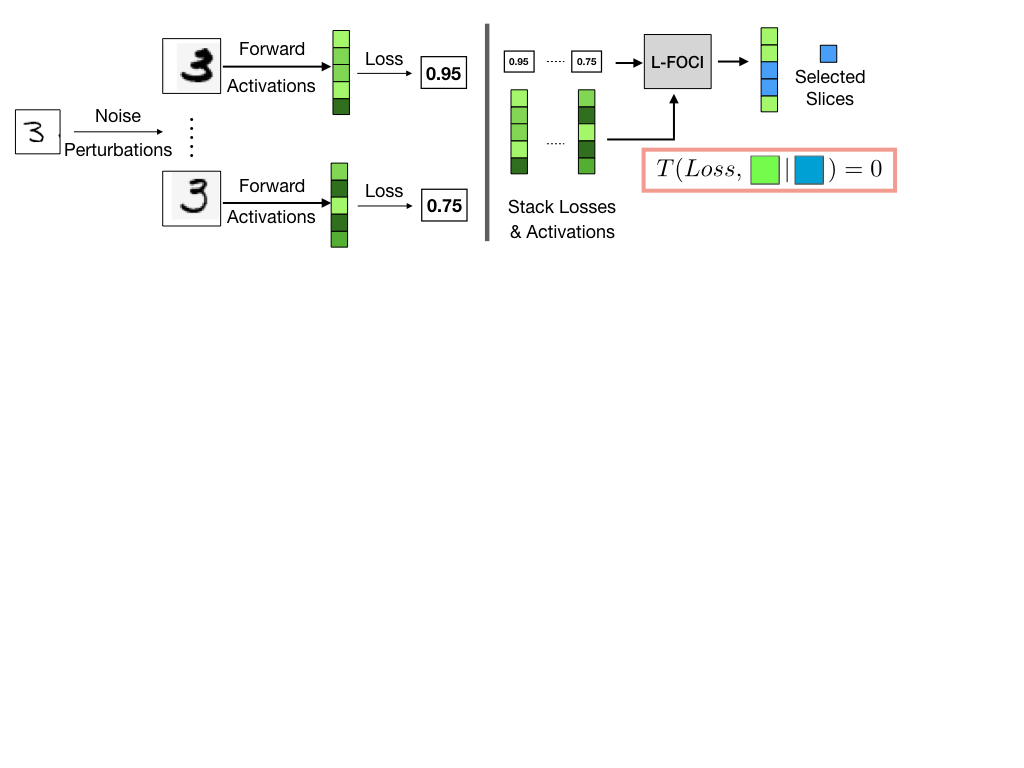
\includegraphics[width=\columnwidth,trim={0 18cm 4cm 0},clip]{5_unlearn/figs/foci_fig_new.png}
    % \vspace{-10pt}
    \caption{A sample is perturbed and passed through the network. Activations are aggregated alongside losses and fed to L-FOCI. Selected rows represent slices of the corresponding layer that are sufficient for unlearning.}
    \label{fig:lfoci}
\end{figure}

When using L-CODEC, we can use a more straightforward Markov Blanket identification procedure adapted from \cite{codec}. FOCI more directly selects which variables are valuable for explaining $z'$, and in fact, is proven to identify the sufficient set (Markov Blanket) with a reasonable number of samples. Briefly, in our L-FOCI, the sufficient set is built incrementally with successive calls to L-CODEC, moving the most ``dependent'' feature from the independent set to the sufficient set.
\todo{See appendix for details.}
% Additionally,they provide a simple procedure for sufficient subset selection, reproduced in Algorithm~\ref{alg:foci}.

\paragraph{Summary.} This procedure alleviates the first issue in terms of sufficient subset or Markov Blanket selection; compared to existing methods using information-theoretic measures that require permutation testing, L-FOCI directly estimates the change in variance when considering a proposal to add to the set.
Now, we discuss how this selection can help identify sets of parameters that can be updated.
